\documentclass[twocolumn,pra,floatfix]{revtex4-2}
\usepackage{amssymb}
\usepackage{amsfonts}
\usepackage{amsmath}
\usepackage{amsxtra}
\usepackage{amscd}
\usepackage{amsthm}
\usepackage{graphicx}
\usepackage{float}
\usepackage{subfig}
\captionsetup[subfloat]{labelformat=empty, captionskip=0pt, farskip=4pt, nearskip=0pt}
% sub-figure with its (a)/(b) marker overlaid in the top-left corner of the image
\newcommand{\panel}[3][\linewidth]{\subfloat[]{\label{#2}\begin{tikzpicture}
    \node[inner sep=0, anchor=north west] (img) at (0,0) {\includegraphics[width=#1]{#3}};
    \node[anchor=north west, inner sep=3pt, font=\bfseries] at (img.north west) {(\thesubfigure)};
\end{tikzpicture}}}
\renewcommand{\topfraction}{0.9}
\renewcommand{\bottomfraction}{0.9}
\renewcommand{\textfraction}{0.1}
\renewcommand{\floatpagefraction}{0.8}
\usepackage{epsf}
\usepackage{bbold}
\usepackage{xcolor}
\usepackage{mathalfa}
%\usepackage{showlabels}
\usepackage{eucal}
\usepackage{bm}
\usepackage{array}
%\usepackage{dcolumn}
\usepackage{hyperref}
\usepackage{xcolor}
\usepackage{tikz}
\usepackage{lipsum}
\hypersetup{
    colorlinks=true,
    linkcolor=blue,
    filecolor=blue,      
    urlcolor=blue,
    citecolor=blue,
    }

\begin{document}

  
    \begin{titlepage}      
        \begin{center}
            
\includegraphics[width=2.5cm]{figures/lu_logo.png}\\[0.3cm]
            {\LARGE Lancaster University\\[0.3cm]
            Department of Physics\par}
            \vspace{0.6cm}

            {\huge\linespread{1.2}\selectfont Creating Classification Neural Networks from Mathematical Principles\par}
            \vspace{0.4cm}

            {\huge Machine Learning C\par}
            \vspace{0.6cm}
			%{\color{blue} \rule{\textwidth}{1pt}}

            {\Large Amelia McCormack, Connor Pochin, Flaka Tahiri, Joe Pickersgill, and Sam Hudson-Oldroyd\par}
            \vspace{0.3cm}

            {\large \emph{Module:} PHYS379\par}
            \vspace{0.6cm}

            {\date{December 2024}}

            \begin{minipage}{0.92\textwidth}
                \small
                \setlength{\parindent}{1.5em}
                \centerline{\textbf{Abstract}}\medskip
                Utilising neural networks and language processing models is crucial in the fields of machine learning and artificial intelligence. These taught algorithms have had positive applications in almost every scientific sector, tracking patterns, processing large amounts of data, and making predictions. In this study, we have developed our own neural networks for characterizing handwritten characters as well as our own language model which will classify books by genre based on their descriptions.

                In this report we will formulate the mathematical foundation and explain the function of both fully connected neural networks and convolution neural networks. Here, we analyse how the performance of the neural network responds to changes to the initial user-chosen parameters and activation functions. The success of the neural networks will be assessed based on its ability to generalise to unseen validation data, and the metrics which quantify performance are: loss and accuracy. We also included two different optimisation algorithms: Adam and stochastic gradient descent, and compared how the neural networks performed when each were implemented. The training and validation sets consist of data from the MNIST dataset (handwritten numbers and lowercase letters), mathematical symbols from an adapted version of the CHROME dataset. Data from the Open Library which provided us with both the descriptions of books and their associated genres.

                We also explore how the use of differing embedding techniques used when processing data can affect the performance of the neural network by means of its accuracy as it evolves as the number of epochs increases. The two embedding techniques we looked at for this project were Doc2Vec and SBERT. Doc2Vec is a model that we trained ourselves on the descriptions of  books sourced from the Open Library while SBERT is a pre-trained model. The comparisons we can draw from using these two separate embedding techniques will inform us as to which one was more effective when used in tandem with our neural network.

                We found that tuning the initial values of the user-chosen parameters was pivotal to yielding a stable accuracy and achieving convergence of the loss function. For he image classification sub-project, the convolution neural network displayed the most successful performance, achieving an accuracy of 98\% on the MNIST validation dataset when the initial learning rate was set to 0.005. Unsurprisingly, the convolution neural network also showed the best performance on the mathematical symbol dataset achieving a final validation accuracy of 90\%. For genre classification, we deemed SBERT to be the better embedding technique as it yielded the result of 94\% validation accuracy while Doc2Vec reached 92\% both after 10 epochs and using the Adam optimiser with initial leaning rate 0.01.


            \end{minipage}
        \end{center}
    \end{titlepage}


    \title{TITLE}
    \author{Amelia McCormack, Connor Pochin, Flaka Tahiri, Joe Pickersgill, and Sam Hudson-Oldroyd}

    % revtex's titlepage doesn't end the page in two-column mode, so force the breaks
    \onecolumngrid
    \clearpage
    \tableofcontents
    \clearpage
    \twocolumngrid

    % block paragraphs: a full blank line between paragraphs, no indent
    \setlength{\parindent}{0pt}
    \setlength{\parskip}{\baselineskip}
    \raggedbottom % keep every paragraph gap the same rather than stretching them to fill columns
    % headings already get \parskip above and below, so trim revtex's own heading spacing to match
    \makeatletter
    \renewcommand{\section}{\@startsection{section}{1}{\z@}{0.4cm \@plus1ex \@minus .2ex}{1pt}{\normalfont\small\bfseries}}
    \renewcommand{\subsection}{\@startsection{subsection}{2}{\z@}{0.4cm \@plus1ex \@minus .2ex}{1pt}{\normalfont\small\bfseries}}
    \renewcommand{\subsubsection}{\@startsection{subsubsection}{3}{\z@}{0.4cm \@plus1ex \@minus .2ex}{1pt}{\normalfont\small\itshape}}
    \makeatother

    \section{Introduction}

        % In a world where there is more written and digital data than ever, more data than humans could ever possibly process in any meaningful way, unique problems arise. It is becoming ever difficult to safeguard information, specifically handwritten documents, to classify information and more generally, be able to access information readily and accurately.
        % \\
        % Machine learning techniques, through the use of neural networks and other algorithms, make these seemingly insurmountable tasks manageable.
        % \\
        % Lit review - stuff that has been done before
        % highlight limitations.
        % \\
        % Our project aims to develop machine-learning models that are computationally efficient, accurate, and at the forefront of technology. We aim to develop a neural network that can identify handwritten characters to a high degree of accuracy which could be used to digitise documents as well as use mathematical data so it is also able to process mathematical symbols and digitize equations. 
        % \\
        % This technology is useful across the board, whether it be for information conservation i.e scanning and reading old documents, or for educators wanting to handwrite mathematical equations to be typed up.
        % \\
        % The other side of our projects relates to language processing. We will be determining the success of a Bag Of Words approach to classify book genres based on the description of the book. This technology could make it easy to browse books based on one genre or other attribute.
        % \\
        % It could also easily be applied to other forms of text classification such as within the realms of different types of scientific papers or legal documents.
        % \\
        % We will be developing these machine learning models, analysing the trade-offs in terms of: accuracy, efficiency, applicability, and computational/environmental cost.
        % \\
        % In order to achieve this we will be using training and testing datasets to assess the accuracy of both our neural network and our language model using different algorithms and approaches. The neural network will utilize the MNIST/EMNIST datasets as well as the 'maths' dataset and out own collected data. The BOW model will utilize the Open Library dataset of book descriptions.
        % \\
        % HISTORY

        In a world where there is more data than humans could possibly process in any meaningful way, unique problems arise. It is becoming ever more difficult to safeguard information, specifically handwritten documents, to classify information and more generally, be able to access information readily and accurately. 

        %Neural networks

        %History
        
        Our project has been split into two main individual work packages, both with the goal of developing a training our own neural network. The first of these primary work packages was to adopt a natural language processing (NLP) model in order to determine the genre of any given book based on a description limited to $500$ words. This technology could make it easy to browse books based on one genre or other attribute. It could also easily be applied to other forms of text classification such as within the realms of different types of scientific papers or legal documents. We then compared the effects of two different embedding techniques, Doc2Vec and SBERT (Sentence Bidirectional Encoder Representations from Transformers). The former being a model that we must train ourselves with our own data while the latter is a pre-trained model. 
        
        Our second primary work package involved, again, developing and training our own neural network. This could be used to digitise documents as well as use mathematical data so it is also able to process mathematical symbols and digitize equations. This technology is useful across the board, whether it be for information conservation i.e scanning and reading old documents, or for educators wanting to handwrite mathematical equations to be typed up. This time to identify handwritten mathematical symbols, numbers and letters. For this classification we compared the effectiveness of different model architectures, Fully Connected Neural Networks (FCNN) and Convolution Neural Networks (CNN). 
        
        As a secondary work package, we compared the effects of different activation functions, specifically the ReLU, Sigmoid and Tanh functions and how the efficiency of the neural network is dependent on which activation functions are used in the hidden layers of the neural network and what their initial parameters are. From here, we aimed to measure the accuracy and efficiency of each of our neural networks as that provides the best indicator as to its performance.

        The foundation of the discovery that was neural networks came from the first use of back propagation in 1976 via the "Taylor expansion of accumulated rounding errors"\cite{nn}.
        This was a key development employed  later in 1982 where back propagation was applied to the first artificial neural network in the work titled "Applications of advances in nonlinear sensitivity analysis"\cite{grad-desc}.
        The next big step in neural networks, convolutional neural networks were discovered in 1998 in a paper named "Gradient-based learning applied to document recognition"\cite{cnn}; this revolutionised computer image recognition. The paper demonstrated one of the first successful CNNs for recognising handwritten input data.

    \section{Background on Machine Learning}

        Machine learning is a subfield of artificial intelligence that enables machines to perform tasks better without explicit programming by using statistical models to draw conclusions from patterns in data. There are 3 distinct types of machine learning: supervised learning, unsupervised learning and reinforcement learning.

        Supervised learning includes a training phase where the model is fed labelled input data. The characteristics of the input data are called features and the supervised learning model uses the data's features and corresponding labels to learn patterns and predict outcomes. Once the model is fully trained, it can be generalized to take in unseen test data and the accuracy can be evaluated by comparing the model’s predictions with correct labels. Supervised learning refers to a learning style that can be divided into two categories: classification and regression. The difference is that the output labels for classification take discrete values whereas the output labels for regression take continuous values. Unsupervised learning is the input data is not labelled, and the algorithm is tasked to find patterns and insights in the data without instruction. An example of an unsupervised learning technique is clustering where unlabelled data points are grouped based on commonality. Reinforcement learning teaches a program to make decisions based on a reward and punishment scheme. After interacting with its environment, it receives feedback from its actions and over time maximizes reward.
        
        Machine learning algorithms can analyse large amounts of data and gain insights from the data that humans can’t notice. These insights can be used to inform business decisions and make predict future trends based on past data. Machine learning has important applications in various fields such as healthcare and finance. A neural network is a common machine learning model loosely based on the neurological functions of the brain. It functions using connected nodes called ‘artificial neurons,’ which process and pass information through a series of layers. The input layer is followed by a series of hidden layers. These layers perform complex transformations and feature extraction. the specifics of these hidden layers will be discussed in the next section.

    \section{Mathematical Background \label{math section}}
    
        \subsection{Introduction}

            Our neural network code is created with a modular design, where each layer of the network is an instance of its respective layer class, which inherits from the base class \texttt{Layer}. This allows for quick and easy creation and changes to the network architecture. To achieve this, however, we need to compute the loss gradient with respect to each layer regardless of the layer that came before it. We find that the chain rule tells us that all we need to compute the gradient of a given layer is the output gradient of that layer. We can show this by the equation,
            \begin{equation}
                \frac{\partial L}{\partial \mathbf{\theta}} = \frac{\partial L}{\partial \mathbf{Y}_i} \frac{\partial \mathbf{Y}_i}{\partial \mathbf{\theta}}
            \end{equation}
            where $L$ is the loss function, $\mathbf{Y}_i$ is the output of layer $i$ and $\theta$ is a trainable parameter. Since for layer $i$, the output $\mathbf{Y}_i$ is equal to the input $\mathbf{X}_{i+1}$ of the next layer $i+1$. We also need to compute the input gradient with respect to each layer and return it for use of the previous layer, for which it becomes the output gradient. 
            \begin{equation}
                \frac{\partial L}{\partial \mathbf{Y}_i} = \frac{\partial L}{\partial \mathbf{X}_{i+1}} 
            \end{equation}
            \begin{figure*}
                \centering
                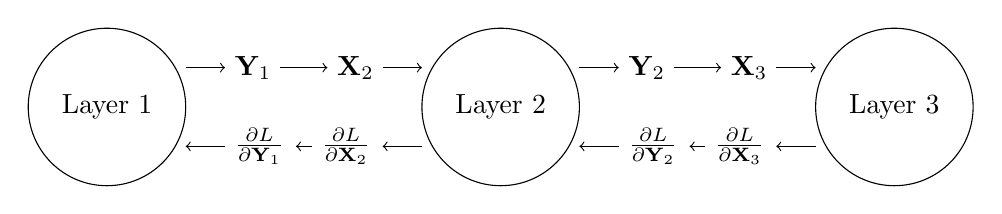
\begin{tikzpicture}
                    % Define nodes
                    \node[circle, draw, minimum size=2cm] (A) at (0,0) {Layer 1};
                    \node[circle, draw, minimum size=2cm] (B) at (5,0) {Layer 2};
                    \node[circle, draw, minimum size=2cm] (C) at (10,0) {Layer 3};

                    % Connect nodes 1-2 forward
                    \draw[->] (1,0.5) -- (1.5,0.5) node[right] {$\mathbf{Y}_1$};
                    \draw[->] (2.2,0.5) -- (2.8,0.5) node[right] {$\mathbf{X}_2$};
                    \draw[->] (3.5,0.5) -- (4,0.5);

                    % Connect nodes 2-3 forward
                    \draw[->] (6,0.5) -- (6.5,0.5) node[right] {$\mathbf{Y}_2$};
                    \draw[->] (7.2,0.5) -- (7.8,0.5) node[right] {$\mathbf{X}_3$};
                    \draw[->] (8.5,0.5) -- (9,0.5);

                    % Connect nodes 3-2 backward
                    \draw[<-] (6,-0.5) -- (6.5,-0.5) node[right] {$\frac{\partial L}{\partial \mathbf{Y}_2}$};
                    \draw[<-] (7.4,-0.5) -- (7.6,-0.5) node[right] {$\frac{\partial L}{\partial \mathbf{X}_3}$};
                    \draw[<-] (8.5,-0.5) -- (9,-0.5);

                    % Connect nodes 2-1 backward
                    \draw[<-] (1,-0.5) -- (1.5,-0.5) node[right] {$\frac{\partial L}{\partial \mathbf{Y}_1}$};
                    \draw[<-] (2.4,-0.5) -- (2.6,-0.5) node[right] {$\frac{\partial L}{\partial \mathbf{X}_2}$};
                    \draw[<-] (3.5,-0.5) -- (4,-0.5);
                \end{tikzpicture}
                \caption{\emph{Forward and backward pass of a neural network.}}
                \label{fig:forward_backward}
            \end{figure*}
            
        \subsection{Fully Connected Layer}
        
            \subsubsection{Forward Propagation}
            
                Our dense or fully connected layer forward propagation is defined by the equation,
                \begin{equation}
                    \mathbf{Y} = \mathbf{W} \mathbf{X} + \mathbf{B}\label{eq:5}
                \end{equation}
                where $\mathbf{X}$ is the input, $\mathbf{W}$ is the weight matrix, $\mathbf{B}$ is the bias vector, and $\mathbf{Y}$ is the output. The weight matrix is of size $n \times m$ where $n$ is the number of output features and $m$ is the number of input features. The bias vector is of size $m$. If the input matrix is of size $m \times k$ where $k$ is the number of samples, then the output matrix is of size $n \times k$. We can write the $i$-th element of the $b$-th output vector in a batch of outputs as,
                \begin{equation}
                    y_i^{[b]} = \sum_{j=1}^{n} w_{i,j} x_j^{[b]} + b_i.
                    \label{eq:paticular_output}
                \end{equation}    
                
            \subsubsection{Loss Gradient with respect to the Weight Matrix}
            
                The error gradient with respect to the weight matrix is given by \cite{Bendersky2018},
                \begin{equation}
                    \frac{\partial L}{\partial \mathbf{W}} = \frac{\partial L}{\partial \mathbf{Y}} \frac{\partial \mathbf{Y}}{\partial \mathbf{W}}.
                \end{equation}
                Within our backward propagation method, we are given the output gradient $\frac{\partial L}{\partial \mathbf{Y}}$ as an argument. This leaves us to compute $\frac{\partial \mathbf{Y}}{\partial \mathbf{W}}$. For any particular element of the gradient $\frac{\partial \mathbf{Y}}{\partial \mathbf{W}}$ we can substitute equation \ref{eq:paticular_output} into the equation,
                \begin{equation}
                    \frac{\partial y^{[b]}_t}{\partial w_{i,j}} = \frac{\partial}{\partial w_{i,j}} \left( \sum_{j=1}^{n} w_{t,j} x_j^{[b]} + b_t \right) = 
                    \begin{cases}
                        x_j^{[b]} & \text{if } i = t \\
                        0 & \text{otherwise}
                    \end{cases}
                    \label{eq:dense_grad_particular}
                \end{equation}
                giving us the gradient of an particular element of $\mathbf{Y}$ with respect to any particular element of $\mathbf{W}$. Representing the gradient of the loss function with respect to the weight matrix as a matrix, we have,
                \begin{equation}
                    \frac{\partial L}{\partial \mathbf{W}} = 
                    \begin{bmatrix}
                        \frac{\partial L}{\partial w_{1,1}} & \frac{\partial L}{\partial w_{1,2}} & \cdots & \frac{\partial L}{\partial w_{1,n}} \\
                        \frac{\partial L}{\partial w_{2,1}} & \frac{\partial L}{\partial w_{2,2}} & \cdots & \frac{\partial L}{\partial w_{2,n}} \\
                        \vdots & \vdots & \ddots & \vdots \\
                        \frac{\partial L}{\partial w_{m,1}} & \frac{\partial L}{\partial w_{m,2}} & \cdots & \frac{\partial L}{\partial w_{m,n}}
                    \end{bmatrix}.
                    \label{eq:dense_grad_matrix}
                \end{equation}
                It follows from equation \ref{eq:dense_grad_particular} that the gradient of the loss function with respect a particular weight $w_{i,j}$ is given by,
                \begin{equation}
                    \frac{\partial L}{\partial w_{i,j}} = \sum_{b=1}^{k} \frac{\partial L}{\partial y^{[b]}_i} x_j^{[b]}.
                    \label{eq:dense_grad}
                \end{equation}
                Substituting equation \ref{eq:dense_grad} into equation \ref{eq:dense_grad_matrix} we find that the final gradient of the loss function with respect to the weight matrix is given by,
                \begin{equation}
                    \frac{\partial L}{\partial \mathbf{W}} = \frac{1}{k}\frac{\partial L}{\partial \mathbf{Y}} \mathbf{X}^T\label{eq:dldw}
                \end{equation}
                where the factor of $\frac{1}{k}$ is used to find the average over the batch.
            \subsubsection{Loss Gradient with respect to the Bias Vector}

                The error gradient with respect to the bias vector is given by,
                \begin{equation}
                    \frac{\partial L}{\partial \mathbf{B}} = \frac{\partial L}{\partial \mathbf{Y}} \frac{\partial \mathbf{Y}}{\partial \mathbf{B}}.
                \end{equation}
                Again, we are given the output gradient $\frac{\partial L}{\partial \mathbf{Y}}$ as an argument, so our task is to compute $\frac{\partial \mathbf{Y}}{\partial \mathbf{B}}$. Referencing equation \ref{eq:paticular_output}, we can see that the gradient of the output with respect to the bias vector is given by,
                \begin{equation}
                    \frac{\partial y^{[b]}_i}{\partial b_j} = \frac{\partial}{\partial b_j} \left( \sum_{j=1}^{n} w_{i,j} x_j^{[b]} + b_i \right) = 
                    \begin{cases}
                        1 & \text{if } i = j \\
                        0 & \text{otherwise}
                    \end{cases}
                \end{equation}
                giving us the gradient of any particular element of $\mathbf{Y}$ with respect to any particular element of $\mathbf{B}$. Representing the gradient of the loss function with respect to the bias vector as a vector, we have,
                \begin{equation}
                    \frac{\partial L}{\partial \mathbf{B}} = 
                    \begin{bmatrix}
                        \frac{\partial L}{\partial b_1} \\[0.5em]
                        \frac{\partial L}{\partial b_2} \\[0.5em]
                        \vdots \\[0.5em]
                        \frac{\partial L}{\partial b_m}
                    \end{bmatrix}.
                \end{equation}
                It follows that the gradient of the loss function with respect to a particular bias $b_i$ is given by,
                \begin{equation}
                    \frac{\partial L}{\partial b_i} = \frac{1}{k} \sum_{b=1}^{k} \frac{\partial L}{\partial y^{[b]}_i}
                \end{equation}
                where the factor of $\frac{1}{k}$ is used to find the average over the batch.
                
            \subsubsection{Loss Gradient with respect to the Input}
            
                The error gradient with respect to the input is given by \cite{Bendersky2018},
                \begin{equation}
                    \frac{\partial L}{\partial \mathbf{X}} = \frac{\partial L}{\partial \mathbf{Y}} \frac{\partial \mathbf{Y}}{\partial \mathbf{X}}.
                \end{equation}
                Referring back to equation \ref{eq:paticular_output}, we can substitute the equation for the output. Hence,
                \begin{equation}
                    \frac{\partial y^{[b]}_i}{\partial x_j^{[b]}} = \frac{\partial}{\partial x_j^{[b]}} \left( \sum_{j=1}^{n} w_{i,j} x_j^{[b]} + b_i \right) = w_{i,j}.
                \end{equation}
                Hence for the $b$-th sample of the input, the error gradient with respect to the input is, 
                \begin{equation}
                    \frac{\partial L}{\partial x^{[b]}_i} = \sum_{j=1}^{n} \frac{\partial L}{\partial y^{[b]}_j} \frac{\partial y^{[b]}_j}{\partial x^{[b]}_i} =
                    \sum_{j=1}^{n} \frac{\partial L}{\partial y^{[b]}_j} w_{j,i}.
                \end{equation}
                We find that this equation can expanded to all samples in the batch and the equation,
                \begin{equation}
                    \frac{\partial L}{\partial \mathbf{X}} = \mathbf{W}^T \frac{\partial L}{\partial \mathbf{Y}}
                \end{equation}
                represents the full gradient of the loss function with respect to the input.
                
        \subsection{Convolutional Layer}
        
            \subsubsection{Forward Propagation}
            
                The convolutional layer is a layer that takes a 3-dimensional input, where the first two dimensions are the height and width of the input (usually pixel values of an image), and the third dimension is the channels of the input. The convolutional layer is defined by the equation \cite{Solai2018},
                \begin{equation}
                    \mathbf{Y}_{i}^{[b]} = \sum_{j=1}^n \mathbf{X}_{j}^{[b]} \ast  \mathbf{F}_{j,i} + \mathbf{B}_{i}
                \end{equation}
                where $\mathbf{Y}_{i}^{[b]}$ is the $i$-th channel of the $b$-th sample of the output, $\mathbf{X}_{j}^{[b]}$ is the $j$-th channel of the $b$-th sample of the input, $\mathbf{F}_{j,i}$ is the $j$-th channel of the $i$-th filter, $\mathbf{B}_{i}$ is the $i$-th bias vector and $\ast$ is the convolution operator. The convolution operator is an operation that takes a filter in the form of a 2d matrix and an in input in the form of a 2d matrix, the filter slides of the input and computes the sum of the element-wise product of the filter and the input. For the example the convolution of a $2 \times 2$ filter and a $3 \times 3$ input is shown below:
                \begin{equation}
                    \begin{bmatrix}
                        x_{1,1} & x_{1,2} & x_{1,3} \\
                        x_{2,1} & x_{2,2} & x_{2,3} \\
                        x_{3,1} & x_{3,2} & x_{3,3} \\
                    \end{bmatrix} \ast
                    \begin{bmatrix}
                        f_{1,1} & f_{1,2} \\
                        f_{2,1} & f_{2,2} \\
                    \end{bmatrix} =
                    \begin{bmatrix}
                        o_{1,1} & o_{1,2} \\
                        o_{2,1} & o_{2,2} \\
                    \end{bmatrix}
                \end{equation}
                where
                \begin{equation}
                    \begin{aligned}
                        o_{1,1} &= x_{1,1}f_{1,1} + x_{1,2}f_{1,2} + x_{2,1}f_{2,1} + x_{2,2}f_{2,2}\\ 
                        o_{1,2} &= x_{1,2}f_{1,1} + x_{1,3}f_{1,2} + x_{2,2}f_{2,1} + x_{2,3}f_{2,2}\\
                        o_{2,1} &= x_{2,1}f_{1,1} + x_{2,2}f_{1,2} + x_{3,1}f_{2,1} + x_{3,2}f_{2,2}\\
                        o_{2,2} &= x_{2,2}f_{1,1} + x_{2,3}f_{1,2} + x_{3,2}f_{2,1} + x_{3,3}f_{2,2}.\\
                    \end{aligned}
                \end{equation}
                
            \subsubsection{Loss Gradient with respect to the Filter}
            
                The loss gradient with respect to the filter is given by,
                \begin{equation}
                    \frac{\partial L}{\partial \mathbf{F}} = \frac{\partial L}{\partial \mathbf{Y}} \frac{\partial \mathbf{Y}}{\partial \mathbf{F}}.
                \end{equation}
                Analysing a simple case with a single kernel, a single input channel and a single sample for a $3 \times 3$ input and a $2 \times 2$ filter, we can see that the elements of the output are given by \cite{Solai2018},
                \begin{equation}
                    \begin{aligned}
                        y_{1,1} &= x_{1,1}f_{1,1} + x_{1,2}f_{1,2} + x_{2,1}f_{2,1} + x_{2,2}f_{2,2} + 
                        b_{11} \\
                        y_{1,2} &= x_{1,2}f_{1,1} + x_{1,3}f_{1,2} + x_{2,2}f_{2,1} + x_{2,3}f_{2,2} + 
                        b_{12} \\
                        y_{2,1} &= x_{2,1}f_{1,1} + x_{2,2}f_{1,2} + x_{3,1}f_{2,1} + x_{3,2}f_{2,2} + 
                        b_{21} \\
                        y_{2,2} &= x_{2,2}f_{1,1} + x_{2,3}f_{1,2} + x_{3,2}f_{2,1} + x_{3,3}f_{2,2} +
                        b_{22}.
                    \end{aligned}\label{eq:22}
                \end{equation}
                Hence, using the chain rule the equation
                \begin{equation}
                    \frac{\partial L}{\partial f_{1,1}} = \frac{\partial L}{\partial y_{1,1}} \frac{\partial y_{1,1}}{\partial f_{1,1}} + \frac{\partial L}{\partial y_{1,2}} \frac{\partial y_{1,2}}{\partial f_{1,1}} + \frac{\partial L}{\partial y_{2,1}} \frac{\partial y_{2,1}}{\partial f_{1,1}} + \frac{\partial L}{\partial y_{2,2}} \frac{\partial y_{2,2}}{\partial f_{1,1}}
                \end{equation}
                represents the gradient of the loss function with respect to the 1st row and 1st column of the filter. Taking the derivatives of the output with respect to the filter, the equation becomes,
                \begin{equation}
                    \frac{\partial L}{\partial f_{1,1}} = \frac{\partial L}{\partial y_{1,1}} x_{1,1} + \frac{\partial L}{\partial y_{1,2}} x_{1,2} + \frac{\partial L}{\partial y_{2,1}} x_{2,1} + \frac{\partial L}{\partial y_{2,2}} x_{2,2}.
                \end{equation}
                Repeating this process for all elements of the filter, we find that the gradient of the loss function with respect to the filter in the general case is given by,
                \begin{equation}
                    \frac{\partial L}{\partial \mathbf{F}_{i,j}} = \sum_{b=1}^{k} \mathbf{X}_{j}^{[b]} \ast \frac{\partial L}{\partial \mathbf{Y}_{i}^{[b]}}
                \end{equation}
                where $F_{i,j}$ is the $i$-th channel of the $j$-th filter, $X_{j}^{[b]}$ is the $j$-th channel of the $b$-th sample of the input, and $Y_{i}^{[b]}$ is the $i$-th channel of the $b$-th sample of the output.
                
            \subsubsection{Loss Gradient with respect to the Bias}

                The loss gradient with respect to the bias matrix is given by,
                \begin{equation}
                    \frac{\partial L}{\partial \mathbf{B}} = \frac{\partial L}{\partial \mathbf{Y}} \frac{\partial \mathbf{Y}}{\partial \mathbf{B}}\label{eq: loss (conv) wrt bias}
                \end{equation}
                Reanalysing the simple case described by the set of equations in \ref{eq:22}, and once again making use of the chain rule
                \begin{equation}
                    \frac{\partial L}{\partial b_{1,1}} = \frac{\partial L}{\partial y_{1,1}} \frac{\partial y_{1,1}}{\partial b_{1,1}} + \frac{\partial L}{\partial y_{1,2}} \frac{\partial y_{1,2}}{\partial b_{1,1}} + \frac{\partial L}{\partial y_{2,1}} \frac{\partial y_{2,1}}{\partial b_{1,1}} + \frac{\partial L}{\partial y_{2,2}} \frac{\partial y_{2,2}}{\partial b_{1,1}}.\label{eq:dldb}
                \end{equation}
                This time, the derivatives of the output with respect to the element in the 1st row and 1st column of the bias matrix satisfy the following equation:
                \begin{equation}
                    \frac{\partial y_{i,j}}{\partial b_{1,1}} = 
                    \begin{cases}
                        1 & \text{if } i, j = 1 \\
                        0 & \text{otherwise}
                    \end{cases}
                \end{equation}
                and therefore equation \ref{eq:dldb} transforms to become
                \begin{equation}
                    \frac{\partial L}{\partial b_{1,1}} = \frac{\partial L}{\partial y_{1,1}}.
                \end{equation}
                Computing the equivalent expressions for all other elements of the bias matrix in this simplified case, the loss gradient with respect to the bias is equal to the loss gradient with respect to the output.

                For the general case therefore, the loss gradient with respect to the bias is given the the equation
                \begin{equation}
                    \frac{\partial L}{\partial \mathbf{B}_i} = \frac{1}{k}\sum_{b=1}^{k} \frac{\partial L}{\partial \mathbf{Y}^{[b]}_i}
                \end{equation}
                where the factor of $\frac{1}{k}$ is used to find the average derivative over the batch.

            \subsubsection{Loss Gradient with respect to the Input}

                The loss gradient with respect to the input is given by,
                \begin{equation}
                    \frac{\partial L}{\partial \mathbf{X}} = \frac{\partial L}{\partial \mathbf{Y}} \frac{\partial \mathbf{Y}}{\partial \mathbf{X}}\label{eq: loss (conv) wrt input}.
                \end{equation}
                Returning to the system of equations (\ref{eq:22}) describing the simplified case with the 3 x 3 input and and 2 x 2 filter, evaluating the derivative of the output with respect to the input unsurprisingly yields a set of nine equations.
                \begin{equation}
                    \begin{aligned}
                        \frac{\partial L}{\partial x_{1,1}} &= \frac{\partial L}{\partial y_{1,1}}f_{1,1}\\ 
                        \frac{\partial L}{\partial x_{1,2}} &= \frac{\partial L}{\partial y_{1,1}}f_{1,2} + \frac{\partial L}{\partial y_{1,2}}f_{1,1}\\
                        \frac{\partial L}{\partial x_{1,3}} &= \frac{\partial L}{\partial y_{1,2}}f_{1,2}\\
                        \frac{\partial L}{\partial x_{2,1}} &= \frac{\partial L}{\partial y_{1,1}}f_{2,1} + \frac{\partial L}{\partial y_{2,1}}f_{1,1}\\
                        \frac{\partial L}{\partial x_{2,2}} &= \frac{\partial L}{\partial y_{1,1}}f_{2,2} + \frac{\partial L}{\partial y_{1,2}}f_{2,1} + \frac{\partial L}{\partial y_{2,1}}f_{1,2} + \frac{\partial L}{\partial y_{2,2}}f_{1,1}\\
                        \frac{\partial L}{\partial x_{2,3}} &= \frac{\partial L}{\partial y_{1,2}}f_{2,2} + \frac{\partial L}{\partial y_{2,2}}f_{1,2} \\
                        \frac{\partial L}{\partial x_{3,1}} &= \frac{\partial L}{\partial y_{2,1}}f_{2,1} \\
                        \frac{\partial L}{\partial x_{3,2}} &= \frac{\partial L}{\partial y_{2,1}}f_{2,2} + \frac{\partial L}{\partial y_{2,2}}f_{2,1}\\
                        \frac{\partial L}{\partial x_{3,3}} &= \frac{\partial L}{\partial y_{2,2}}f_{2,2}.
                    \end{aligned}\label{eq:32}
                \end{equation}
                It is possible to represent the set nine equations as a full convolution operation between a 180-degree rotated filter and the loss gradient with respect to the output. This can be expressed via the following matrix equation
                \begin{equation}
                    \begin{bmatrix}
                        f_{2,2} & f_{2,1} \\
                        f_{1,2} & f_{1,1} \\
                    \end{bmatrix} \ast_{full}
                    \begin{bmatrix}
                        \frac{\partial L}{\partial o_{1,1}} & \frac{\partial L}{\partial o_{1,2}} \\[0.5em]
                        \frac{\partial L}{\partial o_{2,1}} & \frac{\partial L}{\partial o_{2,2}} \\[0.5em]
                    \end{bmatrix} = 
                    \begin{bmatrix}
                        \frac{\partial L}{x_{1,1}} & \frac{\partial L}{x_{1,2}} & \frac{\partial L}{x_{1,3}} \\[0.5em]
                        \frac{\partial L}{x_{2,1}} & \frac{\partial L}{x_{2,2}} & \frac{\partial L}{x_{2,3}} \\[0.5em]
                        \frac{\partial L}{x_{3,1}} & \frac{\partial L}{x_{3,2}} & \frac{\partial L}{x_{3,3}} \\[0.5em]
                    \end{bmatrix}.
                \end{equation}
                Generalising to find the loss gradient with respect to the $j$-th channel of the input 
                \begin{equation}
                    \frac{\partial L}{\partial \mathbf{X}_{j}} = \sum_{b=1}^{k}\sum_{i=1}^{n}rot180(\mathbf{F}_{i,j}) \ast_{full}\frac{\partial L}{\partial \mathbf{Y}_{i}^{[b]}}.
                \end{equation}

        \subsection{Activation Functions}
            
            Activation functions are used to introduce non-linearity into our neural network. We used a total of four activation functions in our code, the ReLU, Sigmoid, Tanh, and Softmax functions. Since all activation functions are not trainable, we only need to compute the input gradient. The input gradient is given by,
            \begin{equation}
                \frac{\partial L}{\partial \mathbf{X}} = \frac{\partial L}{\partial \mathbf{Y}} \frac{\partial \mathbf{Y}}{\partial \mathbf{X}}. 
                \label{eq:input_gradient_activation}
            \end{equation}
            Hence, for each activation function we simply need to compute the derivative of the function with respect to the input.
                
            \subsubsection{ReLU}\label{relu}
            
                The ReLU function is defined as,
                \begin{equation}
                    f(x) = 
                    \begin{cases}
                        x & \text{if } x > 0 \\
                        0 & \text{otherwise}.
                    \end{cases}
                \end{equation}
                Following equation \ref{eq:input_gradient_activation}, the input gradient is given by,
                \begin{equation}
                    \frac{\partial L}{\partial \mathbf{X}} = 
                    \frac{\partial L}{\partial \mathbf{Y}} f'(\mathbf{X}) = 
                    \frac{\partial L}{\partial \mathbf{Y}}
                    \begin{cases}
                        1 & \text{if } x > 0 \\
                        0 & \text{otherwise}
                    \end{cases}.
                \end{equation}
                
            \subsubsection{Sigmoid}\label{sigmoid}
            
                The sigmoid function is defined as,
                \begin{equation}
                    f(x) = \frac{1}{1 + e^{-x}}\label{eq:sig}.
                \end{equation}
                The derivative of the sigmoid function is given by,
                \begin{equation}
                    f'(x) = f(x)(1 - f(x)).
                \end{equation}
                Hence, the input gradient is given by,
                \begin{equation}
                    \frac{\partial L}{\partial \mathbf{X}} = 
                    \frac{\partial L}{\partial \mathbf{Y}} f'(\mathbf{X}) = 
                    \frac{\partial L}{\partial \mathbf{Y}} f(\mathbf{X})(1 - f(\mathbf{X})).
                \end{equation}
                
            \subsubsection{Tanh}

                The tanh function is defined as,
                \begin{equation}
                    f(x) = \frac{e^x - e^{-x}}{e^x + e^{-x}}.
                \end{equation}
                The derivative of the tanh function is given by,
                \begin{equation}
                    f'(x) = 1 - f(x)^2.
                \end{equation} 
                Hence, the input gradient is given by,
                \begin{equation}
                    \frac{\partial L}{\partial \mathbf{X}} = 
                    \frac{\partial L}{\partial \mathbf{Y}} f'(\mathbf{X}) = 
                    \frac{\partial L}{\partial \mathbf{Y}} (1 - f(\mathbf{X})^2).
                \end{equation}
                
            \subsubsection{Softmax}\label{softmax}

                The softmax function is a unique activation function, that usually is only used on the output layer of a neural network. The softmax function is used to convert the output of a layer into a probability distribution. This is incredibly useful for classification problems. The softmax function is used on a vector of $n$ elements, and is defined as,
                \begin{equation}
                    f(x_i) = \frac{e^{x_i}}{\sum_{j=1}^{n} e^{x_j}}
                \end{equation}
                where $x_i$ is the $i$-th component of the vector and $f(x_i)$ is the probability of the $i$-th component of the vector.
                
        \subsection{Loss Functions}
        
            \subsubsection{Mean Squared Error}
            
                The mean squared error is defined as,
                \begin{equation}
                    L = \frac{1}{k} \sum_{i=1}^{k} \sum_{j=1}^{n} (y_{i,j} - \hat{y}_{i,j})^2\label{eq:loss}
                \end{equation}
                where $k$ is the number of samples, $n$ is the number of output features, $y_{i,j}$ is the $j$-th component of the $i$-th sample, and $\hat{y}_{i,j}$ is the $j$-th predicted component of the $i$-th sample. The derivative of the loss function with respect to the final output ($\mathbf{\hat{Y}}$) is given by,
                \begin{equation}
                    \frac{\partial L}{\partial \mathbf{\hat{Y}}} = \frac{2}{k} (\mathbf{\hat{Y}} - \mathbf{Y}).
                \end{equation}
                The output of this function is then passed to the output layer for back propagation. The mean squared error loss function is used extensively for regression problems.

            \subsubsection{Binary Cross Entropy\label{bce}}
                The binary cross entropy loss function is defined as,
                \begin{equation}
                    L = -\frac{1}{k}\frac{1}{n}\sum^n_{i}\left( y^{[b]}_i 
                    \cdot \log{\hat{y}^{[b]}_i} + (1 - y^{[b]}_i) \cdot 
                    \log{1 - \hat{y}^{[b]}_i} \right) 
                \end{equation}
                where $k$ is the number of samples, $n$ is the number of output features, $y_{i}^{[b]}$ is the $i$-th component of the $b$-th sample, and $\hat{y}_{i}^{[b]}$ is the $i$-th predicted component of the $b$-th sample. The derivative of binary cross entropy with
                respect the output of the final layer is given by,
                \begin{equation}
                    \frac{dL}{d\mathbf{\hat{Y}}} = \frac{\mathbf{\hat{Y}} - \mathbf{Y}}{k(1 - \mathbf{\hat{Y}}) \mathbf{\hat{Y}}}
                \end{equation}
                where the factor of $1/k$ is introduced to average the loss function across the batch. Binary cross entropy is commonly used loss function for classification problems between two (binary) classes.
            \subsubsection{Categorical Cross Entropy}\label{cce}

                The categorical cross entropy loss function is defined as,
                \begin{equation}
                    L = -\frac{1}{k} \sum_{b=1}^{k} \sum_{i=1}^{n} y_{i}^{[b]} \log(\hat{y}_{i}^{[b]})
                \end{equation}
                where $k$ is the number of samples, $n$ is the number of output features, $y_{i}^{[b]}$ is the $i$-th component of the $b$-th sample, and $\hat{y}_{i}^{[b]}$ is the $i$-th predicted component of the $b$-th sample. The cross entropy loss function is used primarily for classification problems with multiple classes. Since the softmax activation function is often found on the output layer of a classification network, it is useful to compute the derivative of the loss function with respect to a softmaxed output. Considering a softmaxed output, the loss function becomes,
                \begin{equation}
                    L = -\frac{1}{k}\sum_{b=1}^{k}\sum_{i=1}^{n}y_{i}^{[b]}\log(\text{Softmax}(z^{[b]}_{i}))
                \end{equation}
                where $z^{[b]}_{i}$ is the $i$-th component of the $b$-th sample of the output of the non-softmaxed output layer. Looking at just the the loss function for a single sample, we can see that the derivative with respect to the output layer is \cite{Kurbiel2021}:
                \begin{align*}
                    L &= -\sum_{j=1}^{n}y_{j}\log(a_{j}) \\
                    \frac{\partial L}{\partial z_{i}} &= - \sum_{j=1}^{n}y_{j}\frac{\partial
                    \log(a_{j})}{\partial z_{i}} \\
                    &= - \sum_{j=1}^{n}y_{j}\frac{1}{a_{j}}\frac{\partial a_{j}}{\partial z_{i}} \\
                \end{align*}
                where $a_i$ is the $i$-th element of the final output of the network and $y_i$ is the i-th element of the label vector. The derivative of the softmax function is:
                \begin{equation}
                    \frac{\partial a_{j}}{\partial z_{i}} = \begin{cases}
                        a_{j}(1-a_{j}) & \text{if } j = i \\
                        -a_{j}a_{i} & \text{if } j \neq i.
                    \end{cases}
                \end{equation}
                Hence:
                \begin{align*}
                    \frac{\partial L}{\partial z_{i}} &= -y_{i}(1-a_{i}) - \sum_{i \neq j}y_{j}a_{i}\\
                                                &= a_{i} \left( y_{i} + \sum_{i \neq j}y_{j} \right) - y_{i} .\\
                \end{align*}
                Since $\sum_{j}y_{j} = 1$, then $y_{i} + \sum_{i \neq j}y_{j} = 1$, we have:
                \begin{equation}
                    \frac{\partial L
                    }{\partial z_{i}} = a_{i} - y_{i}.
                \end{equation}
                We find that
                \begin{equation}
                    \frac{\partial L}{\partial 
                    Z} = \mathbf{\hat{Y}} - \mathbf{Y}
                \end{equation}
                which is the derivative of the loss function with respect to the output of the non-softmaxed output layer, where $\mathbf{\hat{Y}}$ is the final output of the network and $\mathbf{Y}$ is the label vector.
                
        \subsection{Optimization Algorithms}

            \subsubsection{Stochastic Gradient Descent}

                Stochastic gradient descent, or SGD, is the most basic method of optimization. Using the mathematical equations for the loss gradient with respect to the parameter of interest, we can update the parameter to find the optimal solution. SGD is defined by
                \begin{equation}
                    \theta_t = \theta_{t-1} - \alpha \frac{\partial L}{\partial \theta_{t-1}}
                \end{equation}
                where $\theta_t$ is the parameter of interest at timestep $t$, $\alpha$ is the learning rate, and $L$ is the loss function. The learning rate is a 'hyperparameter' defined by the user. SGD is a simple but effective optimization algorithm, however it can be slow to converge and susceptible to becoming trapped in local minima and saddle point. This is due to the inability of SGD to adapt the learning rate during training, and all parameters in the network must share the same learning rate.

            \subsubsection{Adam}\label{Adam}

                The Adam optimization algorithm was first introduced by Diederik P. Kingma and Jimmy Ba in their 2015 paper, "Adam: A Method for Stochastic Optimization". Adam is a much more advanced optimization algorithm than standard SGD, as it uses adaptive learning rates and can tailor the learning rate to each individual parameter. Adam is defined by the equations,
                \begin{equation}
                    \begin{aligned}
                        t &\leftarrow t + 1 \\
                        g_t &\leftarrow \nabla_{\theta} f_t(\theta_{t-1}) \\
                        m_t &\leftarrow \beta_1 m_{t-1} + (1 - \beta_1) g_t \\
                        v_t &\leftarrow \beta_2 v_{t-1} + (1 - \beta_2) g_t^2 \\
                        \hat{m}_t &\leftarrow \frac{m_t}{1 - \beta_1^t} \\
                        \hat{v}_t &\leftarrow \frac{v_t}{1 - \beta_2^t} \\
                        \theta_t &\leftarrow \theta_{t-1} - \alpha \frac{\hat{m}_t}{\sqrt{\hat{v}_t} + \epsilon}
                    \end{aligned}
                \end{equation}
                where $t$ is the timestep, $\theta$ is the parameter of interest, $f_t$ is the loss function at timestep $t$, $\alpha$ is the learning rate, $\beta_1$, $\beta_2$ and $\epsilon$ are hyperparameters set by the user. Adam uses the idea of momentum, which allows the algorithm to 'roll' its way out of local minima and saddle points to find the global minima. Adam also converges much faster than SGD as the learning rate is varied at each timestep, becoming exponentially smaller as the algorithm converges. This allows Adam to make large steps initially and then smaller steps as the algorithm works out the fine details to converge on the global minima.

    \section{Methods}

        \subsection{Code Design}

            We took an object-oriented approach to the code design of our neural 
            networks. As discussed in section \ref{math section}, we first created
            a framework in which networks could easily be created and adjusted as
            needed. To achieve this, we implemented each layer discussed in
            section \ref{math section} as a class which inherited from a base
            class called '\texttt{Layer}'. Each layer class was required to
            implement the '\texttt{prop}' and '\texttt{back\_prop}' methods
            which propagated and backward propagated the given input, 
            respectively. Trainable layers were designed with an initialisation function
            which took a choice of optimizer, hyper-parameters and input size as arguments
            and then initialised their weights and biases randomly and stored them as
            class attributes to be used by the '\texttt{prop}' method and updated by the
            '\texttt{back\_prop}' method. The '\texttt{prop}' method was implemented to
            take an input as an argument and return the propagated output of the layer.
            The '\texttt{back\_prop}' method was implemented to take the derivative of the
            loss function with respect to the output of the layer as an argument and
            return the derivative of the loss function with respect to the input of the layer. We then created a '\texttt{Network}' class which was initialised with a 
            list of layer instances in the specific order in which the model 
            would propagate them. The list would then be stored as a class
            attribute.

            The propagation of a network was implemented in the '\texttt{predict}'
            method of the '\texttt{Network}' class. This method takes an input as the argument and iterates through the list of layers, 
            calling the '\texttt{prop}' method of each layer. The argument given
            to the '\texttt{prop}' method is a variable '\texttt{x}'. '\texttt{x}'
            is initialised to the input of '\texttt{predict}' and updated to be 
            the return output of each '\texttt{prop}' call (see figure
            \ref{fig:forward_backward}). The return value of the final element 
            of the layers list prop method is then returned as the final 
            prediction.

            The backward propagation of a network was implemented in the 
            '\texttt{backward}' method of the '\texttt{Network}' class. This method first 
            called the '\texttt{predict}' method to find the predicted output of the
            network  $\mathbf{\hat{Y}}$. The derivative of the given loss function with
            respect to $\mathbf{\hat{Y}}$ is then found. The method then iterates 
            through a reversed list of the layers, calling the '\texttt{back\_prop}'
            method of each layer. The argument given to the '\texttt{back\_prop}' method
            is a variable '\texttt{dy}'. This variable is initialised as the derivative of
            the loss function with respect to $\mathbf{\hat{Y}}$ and updated to be the 
            returned output of each '\texttt{back\_prop}' call.

            To train the network we implemented a method '\texttt{train}' in the 
            \texttt{Network} class. This method takes labelled training data, number of 
            epochs, batch size and labelled validation data as arguments. When called, the 
            method first splits the training data into 'batches' defined by the batch size.
            The method then loops through each epoch. During the epoch the method loops
            through the batches calling the '\texttt{backward}' method for each loop and
            providing the batch as an argument. The method then computes the accuracy 
            between the predicted labels $\hat{y}$ and the actual labels $y$ and stores 
            these values in a class attribute for later use. At the end of each epoch 
            predictions for the validation data labels are made using the 
            '\texttt{predict}' method and accuracy of the model is again computed and
            stored in a class attribute. The training data is also randomly shuffled 
            between epochs. This is done to decrease the likelihood of over-fitting
            during training.

            Our code is dependent on a number of libraries for various functionality,
            such as 'numpy' \cite{numpy} for linear algebra, 'scipy' \cite{scipy} for 2D
            convolution calculations, 'matplotlib' \cite{matplotlib} for plotting
            figures, 'PIL' \cite{pillow} for image processing, and 'pandas' \cite{pandas} for data processing. We also used PyTorch's functional library \cite{torch} for our Max-Pooling layer, we felt this was acceptable as pooling layers are non-trainable and primary used to reduce computational power.

        \subsection{Book Genre Classification}

            We chose to use the description of a book to predict the genre in order to determine whether there is a correlation between the vocabulary that is used when describing a book and and its genre. 
    
            In order for us to train the machine learning algorithm to determine genre from a description, we needed to source a dataset which provides a description of the book and a list of genres the book would be categorised into. The Open Library works edition\cite{openlibrary2025-fullworks} was chosen as our dataset as it provides both a description of each book and a list of subjects in which genres could be found. In order to select appropriate genres, each subject from the Open Library dataset was counted and listed in order of most appearances to least. From the list, nine of the most common subjects that could be interpreted as genres were chosen: history; fantasy; drama; mystery; science fiction; romance; coming of age; action \& adventure; horror. 

            The original dataset from Open Library was then filtered to remove all data that would not be of use to our project by in three steps. The first which limited the data to only include books that listed fiction in the subjects to ensure that we train our algorithm solely on fictitious works. The second step was to check each book in the dataset for at leat one of the nine genres chosen, removing all others as to not provide unnecessary data for the algorithm that could negatively affect its performance. The third step of filtering involved removing entries that did not provide data for the description. These steps filtered down the raw file from Open Library to a set of 43893 books.

                We created a way to vectorise our list of classes: "History"; "Fantasy"; "Drama"; "Mystery"; "Science fiction"; "Romance"; "Fiction, coming of age"; "Fiction, horror"; "Fiction, action \& adventure". By creating a label vector, we can assign a nine dimensional vector to describe the genres that appear in the book's subject list. For each genre that appears in our class, the vector has a value of $1$ in the genres respective position and $0$ in all other positions for those which do not appear. For example the vector
                \begin{align*}
                    \begin{bmatrix}
                         1,0,0,1,0,0,0,0,0
                    \end{bmatrix}
                \end{align*}
                refers to a book which has both the genres history and mystery appear in its subjects list and no others. In order to restrict the bias of excessively long descriptions, we limited each description to 500 words. Each description was tokenised using '\texttt{nltk.work\_tokenize}'\cite{nltk} and collected in a list, thus creating our dataset. For example, this would convert \emph{"a long time ago in a galaxy far far away"} into:
                \begin{align*}
                    \begin{bmatrix}
                        \text{a},\text{long},\text{time},\text{ago},\text{in},\text{a},\text{galaxy},\text{far},\text{far},\text{away}
                    \end{bmatrix}.
                \end{align*}
                
                The first of our two embedding techniques we chose to employ was Doc2Vec\cite{doc2vec-paper}, an unsupervised model which can be used to convert text into a numerical based vector. We trained for $30$ epochs with a vector size of 256 and a window size of 4. Once trained, we could use the Doc2Vec model to vectorise each tokenised book description. However, the performance of Doc2Vec is reliant on the size of the data we train it on. In order to observe these limitations directly, the second embedding technique we used was a pre-trained from SBERT\cite{sbert_models} called '\texttt{all-distilroberta-v1}' which also created a vector for each book description. This model was trained on a larger and more varied set of data which totalled 160GB of text in size.

            \subsubsection{Model Architecture}
    
                The main model of this neural network consisted of hidden four layers: a dense layer; an activation layer; a second dense layer and a second activation layer. It was trained using the the vectors obtained from our embedding techniques, Doc2Vec and SBERT, as the input and its corresponding label vector as its output. The SBERT model was inputed as 768 dimensional vectors while the Doc2Vec model gave us 256 dimensional vectors. The first dense layer took the respective vector from either Doc2Vec or SBERT and transformed it into a vector with 128 dimensions while applying the Adam optimiser (section \ref{Adam}) with initial conditions 0.01 for alpha, 0.9 for beta1 and 0.99 for beta2. The first activation layer used the ReLU function (section \ref{relu}), setting all negative values that appear to zero. Further reducing the size of the vector, the second dense layer brings the vector from 128 dimensions to 9, the same as our label vector while again applying the Adam optimiser with the same conditions as stated previously. Finally, the second activation layer used the Sigmoid function (section \ref{sigmoid}) which gives a probability for each class as an output as well as the binary crossentropy function (section \ref{bce}). This allows each class to be predicted separately for each book as books could belong to multiple genres in our class in a binary yes or no format; an output that is either rounded to 1 or 0 respectively.

        \subsection{Handwriting Recognition}
        
            \subsubsection{Handwriting Datasets}
    
                Standardized large datasets play a crucial role in machine learning, and the MNIST database\cite{lecun2010mnist} (Modified National Institute of Standards and Technology database) is perhaps the most famous. Handwritten digit and character recognition are hugely important for computer vision and pattern recognition. The MNIST dataset has become a benchmark for testing the efficiency of image processing systems and image recognition algorithms. The MNIST database consists of 70,000 images of handwritten digits of 10 classes (0 to 9). 60,00 of these images are used for training and the other 10,000 are used for testing purposes. These black and white images are processed by normalizing them to fit into a 28x28 pixel bounding box to improve model efficiency and they are also anti-aliased; this introduces grey scale levels. The original database known as the NIST database was created in the 80s by the National Institute of Standards and Technology. The MNIST dataset is a modified version of the NIST (M-NIST) handwritten digit database, which was developed by the National Institute of Standards and Technology (NIST) in the 1980s.

                The main aim of our handwriting recognition model was to recognise handwritten mathematical symbols. We decided to use an adapted version of the CROHME dataset. The adapted CROHME dataset features more than 360,000 42x42 PNG images of 82 unique mathematical symbols. We chose to use 80\% of the images as training data and 20\% of the images as testing data.

                % \begin{figure}[h]
                %     \begin{center}
                %         \includegraphics[width=6cm]{mnist.png}\\[0.5cm]
                %         \caption{\emph{Examples of MNIST dataset}}
                %     \end{center}
                % \end{figure}


                % NIST's original data set used Census Bureau employees as the training data, and the test set consisted of samples from American high school students. One improvement made to the MNIST database was to 're-mix' this data to make it more suitable for machine learning models. Half of the training data was changed to testing data, and vice versa. 

                %Historically, MNIST has played a crucial role in advancing computer vision research and deep learning techniques.

                %The final improvement made to the MNIST database was the introduction of handwritten lowercase and uppercase letters.

                %The EMNIST (Extended-MNIST) database contains an impressive 814,255 handwritten uppercase and lowercase letters and digits in the same form as the MNIST database.

                %We decided to make use of these datasets as they provide a large bank of already clean and accurate data to train the algorithm on.

                %The final piece of the puzzle came in the form of the NAME HERE dataset of handwritten mathematical symbols found on GitHub. We wanted to expand the research into handwritten mathematical symbols because currently there is not much technology out there able to recognise these. The would be immensely useful to scientists, students and teachers everywhere.

            %\subsubsection{Data Collection}
        
                %Although the dataset is large and clean we did however run into the issue that for some symbols there were huge amounts of data for whereas others were extremely lacking.

                %In order to combat this we decided to collect some of our own data as well. We did this using SAM EXPLAIN SURVEY CODE.

                %The link to the website was shared through friends and family, word of mouth, and social media. This provides us with varied data from both physicists and non-physicists. In the end we collected NUMBER of samples.

                %PROBLEMS FACED
            \subsubsection{Data Pre-processing}
                To provide the model with usable data and to improve the performance of the model, we applied some pre-processing to the data. The MNIST dataset was acquired as two csv files, one csv file for training data, and one csv file for testing data. The csv file contained 60,000 and 10,000 rows, respectively, and 785 columns. Each row represented an image; the first column represented the label of the image (0-9) and the remaining 784 represented the pixel values of each of the 784 pixels. Each pixel value was an integer value between 0 and 255, where 0 represents a completely black pixel and 255 represents a completely white pixel. The csv files were read by pandas and then turned in numpy arrays. Each label was separated and turned into a one hot encoded vector. One hot encoding is a method that turns an integer into a vector with a single 'hot' dimension. For example, the integer 2 would be represented as [0,0,1,0,0,0,0,0,0,0]. These label vectors were joined to make two 2D tensors of size $10 \times 60,000$ for the training data and $10 \times 10,000$ for the testing data. The pixel values were also joined and transposed to form two 2D tensors of size $784 \times 60,000$ for the training data and $784 \times 10,000$ for the testing data. The image tensors were then normalized by dividing both tensors by $255$, ensuring that the maximum value in each tensor was $1$.

                \begin{table}
                    \centering
                    \footnotesize
                    \renewcommand{\arraystretch}{1.2}
                    \setlength{\tabcolsep}{1.6pt}
                    \begin{tabular}{|c|c|c|c|c|c|c|c|c|c|}
                        \hline
                        \textbf{Label} & \textbf{\begin{tabular}{@{}c@{}}Pixel\\1\end{tabular}} & \textbf{\begin{tabular}{@{}c@{}}Pixel\\2\end{tabular}} & \textbf{\begin{tabular}{@{}c@{}}Pixel\\3\end{tabular}} & \textbf{\begin{tabular}{@{}c@{}}Pixel\\4\end{tabular}} & \textbf{\begin{tabular}{@{}c@{}}Pixel\\5\end{tabular}} & \textbf{\begin{tabular}{@{}c@{}}Pixel\\6\end{tabular}} & \dots & \textbf{\begin{tabular}{@{}c@{}}Pixel\\783\end{tabular}} & \textbf{\begin{tabular}{@{}c@{}}Pixel\\784\end{tabular}} \\
                        \hline
                        0 & 0 & 1 & 2 & 3 & 4 & 5 & \dots & 0 & 1 \\
                        1 & 9 & 8 & 7 & 6 & 5 & 4 & \dots & 2 & 3 \\
                        2 & 3 & 4 & 5 & 6 & 7 & 8 & \dots & 4 & 5 \\
                        \hline
                    \end{tabular}
                    \caption{Example table showing the MNIST csv file.}
                    \label{tab:pixel_table}
                \end{table}
    
                The CROHME dataset was acquired as a compressed folder containing 82 subfolders. Each subfolder represents a class, containing all of the PNG images for that class. To read in the data we iterated through all of the subfolders in the folder, reading in each image in the subfolder with PIL. Each image was then reduced in size using PIL from 42x42 pixels to 28x28 pixels and turned into a numpy array. A one-hot label vector corresponding to the index of the subfolder was created for the image. label and image vectors were then compiled into tensors, creating a 2D tensor of size $784 \times 375,974$ for the images and a 2D tensor of size $82 \times 375,974$ for the labels. The images tensor was also normalized by dividing by $255$. The data were then randomly shuffled and split into training and testing data.
               
            \subsubsection{Model Architecture}
            
                We created two separate models for handwriting recognition. Our simpler model consisted of only fully-connected layers. This model used a single hidden fully connected layer with a ReLU (\ref{relu}) activation function and a fully connected output layer with a softmax (\ref{softmax}) activation function which was used in conjunction with the cross categorical entropy (\ref{cce}) loss function. The hidden layer consisted of a bias vector of size $128$ and weights matrix of size $128 \times 784$ for both datasets, since both datasets were fed to the network as $28 \times 28$ images. The output layer of the network consisted of a bias vector of size $128 \times r$ and weights matrix of size $r \times 128$ where $r$ is the number of classes in the dataset. As mentioned in the previous section for M-NIST dataset $r = 10$, and for the CROHME dataset $r = 82$.

                \begin{figure*}
                    \centering
                    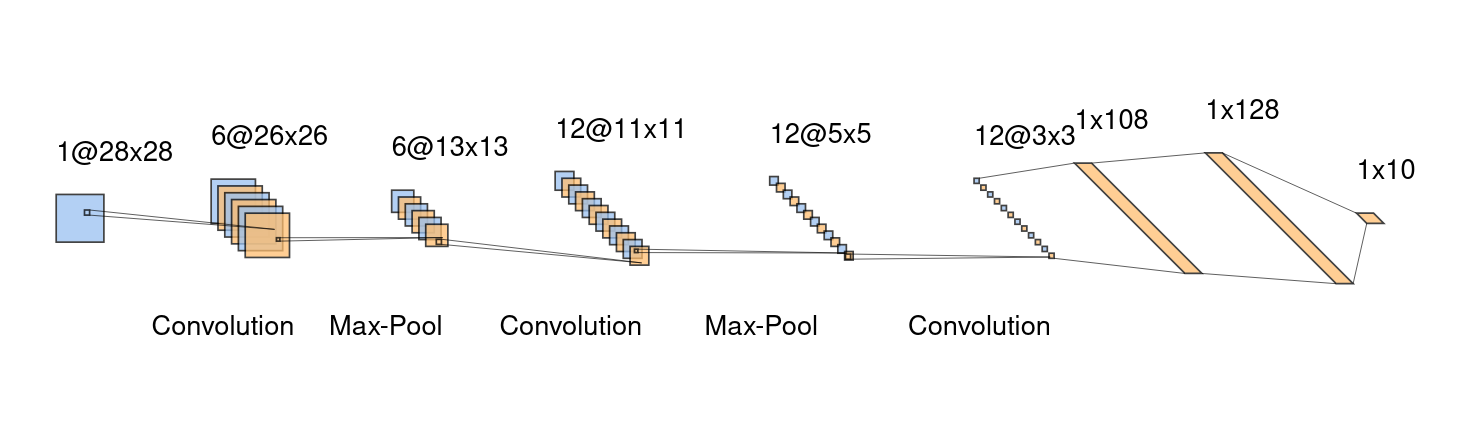
\includegraphics[width=0.8\textwidth]{figures/model_diagram.png}
                    \caption{\emph{Convolutional handwriting recognition neural network architecture.}}
                    \label{fig:math-model}
                \end{figure*}

                Our more complex model was created with 6 hidden layers: 3 convolution layers, 2 pooling layers, and 1 fully connected layers (shown in figure \ref{fig:math-model}). The first convolution layer consisted of 6 filters, while the other two convolution layers consisted of 12 filters. All convolution layers employed a filter size of $3 \times 3$. Both pooling layers consisted of max-pooling with a stride of 2 and filter size of $2 \times 2$. The hidden fully connected layer consisted of a weight matrix of size $128 \times 108$ and a bias vector of size 108. Every trainable hidden layer used the ReLU (\ref{relu}) activation function. Finally, the output layer consisted of a fully connected layer with a weight matrix of size $r \times 128$ and a bias vector of size $r$. The output layer, again, used a softmax (\ref{softmax}) activation function which was used in conjunction with the cross categorical entropy (\ref{cce}) loss function. 
            
    \section{Results}

        \subsection{Performance Analysis of Neural Networks}

            As a method of visualising the training process, we tasked the fully connected neural network to predict data points such that it was able to plot the function $\sin(x)$ on the interval $(0, 2\pi]$. In order to analyse how different activation functions affect the performance of the neural network, it was instructive to plot how the loss function varied as the number of epochs increased. In this section, the mathematical properties of the activation functions are used to explain how the performance differs depending on the choice of activation function for the hidden layers.
            
            The neural network used to generate the sine curve has an input layer, which receives the initial data, three hidden layers and one output layer. Within the hidden layers, weight matrices and bias vectors are applied to the input data as shown in equation \ref{eq:5}, as well as the activation functions being used to introduce non-linearity for propagation. As a way to highlight the difference in performance between the three activation functions: ReLU, Sigmoid and tanh, each sine plot was generated with the same activation function being applied in all three hidden layers of the neural network.

            \begin{figure*}
                \centering
                \panel[0.48\textwidth]{main:a}{figures/sin_ReLu_frame_30000.png}\hfill
                \panel[0.48\textwidth]{main:c}{figures/sin_Tanh_frame_30000.png}
                \caption{\emph{Plots of the function sin(x) on the interval (0, 2$\pi$] generated using ReLU (a) and tanh (b) in the hidden layers of the neural network. The learning rate used for gradient descent was 0.00002 and each plot displays the neural network's predictions after being trained over 30,000 epochs. The predictions made by the neural network are represented by the orange curve, and are plotted on the same axis as the function sin(x) which is represented by the blue curve.}}
                \label{fig:6}
            \end{figure*}

            From a visual standpoint, the neural network's predictions appear to converge to the function sin(x) with appreciable accuracy using ReLU and tanh activation functions, as well as a low learning rate. A quantitative measurement of the model's performance is best achieved by investigating how the loss function varies as the number of epochs increases during the training phase. The loss is calculated using equation \ref{eq:loss}.

            \begin{figure*}
                \centering
                \panel[0.48\textwidth]{fig:7:a}{figures/loss_ReLU_30000.png}\hfill
                \panel[0.48\textwidth]{fig:7:b}{figures/Loss_Tanh_30000.png}
                \caption{\emph{Plot of the natural log of the loss function against the number of epochs when using ReLU (a) and tanh (b) in the hidden layers of the neural network. This is the loss during the training phase as the neural network predicts the function sin(x).}}
                \label{fig:7}
            \end{figure*}

            As displayed in figure \ref{fig:7}, using ReLU, the loss decreases rapidly over the first few hundred epochs until $\ln(L) < -10$, and then decreases steadily until $\ln(L) = -12.5$ over the remainder of the training phase. Comparatively, using tanh as the activation function, $\ln(L)$ is a decreasing function over the entirety of the training phase; reaching a minimum of $\ln(L) = -8$ after the 30,000 epochs. After the first few hundred epochs, $\ln(L) = -4$ and hence the neural network trains much faster using ReLU as opposed to tanh, resulting in superior performance after 30,000 epochs since the final value for $\ln(L)$ is lower using ReLU. 

            The mathematical properties of the activation functions and their derivatives give insights into why ReLU performs better, and trains the neural network much faster than tanh. ReLu is a piecewise functions which is linear for positive inputs and zero for negative inputs; and thus is in keeping with the necessity that the activation functions must introduce non-linearity into the neural network. The derivative of ReLU therefore is the familiar step function. When comparing the derivative of ReLU with the derivative of the hyperbolic tangent, $\text{sech}^{2}(x)$, large inputs ($x >> 1$) are all outputted to 1 when passed into the derivative of ReLU, whereas outputs of $\text{sech}^{2}(x)$ quickly vanish when the input is large. $\text{sech}^{2}(x)$ is an even function and has the same asymptotic behaviour for negative inputs, whereas the step function will output zero for all negative inputs. The loss gradient with respect to the input is passed through the layers during back propagation and given by equation \ref{eq:input_gradient_activation}. For the hidden layers, this is dependent on the derivative of the activation function; and therefore for large positive inputs, the vanishing gradient of tanh leads to smaller updates in the weights and hinders the minimisation of the loss function.
            
            \begin{figure*}
                \centering
                \panel[0.48\textwidth]{fig:8:a}{figures/sin_Sigmoid_frame_10000.png}\hfill
                \panel[0.48\textwidth]{fig:8:b}{figures/sin_Sigmoid_frame_30000.png}
                \caption{\emph{Plots of the function $\sin(x)$ on the interval (0, 2$\pi$] generated using the Sigmoid activation function in the hidden layers of the neural network. The neural networks predictions are displayed after being trained over 10,000 epochs (a) and 30,000 epochs (b), with a learning rate of 0.00002. The predictions made by the neural network are represented by the orange curve, and are plotted on the same axis as the function sin(x) which is represented by the blue curve.}}
                \label{fig:8}
            \end{figure*}
            
            Evidently, from figure \ref{fig:8}, there is very little difference between the predictions made by the neural network after 10,000 epochs and after 30,000 epochs. When compared with ReLU and tanh, we discovered that the predictions made using Sigmoid converge to the sine curve far slower from a visual perspective when examining figures \ref{fig:6} and \ref{fig:8}. The variation of $\ln(L)$ over the 30,000 epochs using Sigmoid (figure \ref{fig:9}) is evidence of this slow convergence. This time, the loss reaches a global minimum of $\ln(L) = -3.5$ after the first few hundred epochs, and is an increasing function for the remainder of the training phase. From 10,000 to 30,000 epochs, the gradient of $\ln(L)$ is positive and shallow; and the loss function fails to reach its minimum value once the training phase has concluded.

            \begin{figure}
                \centering
                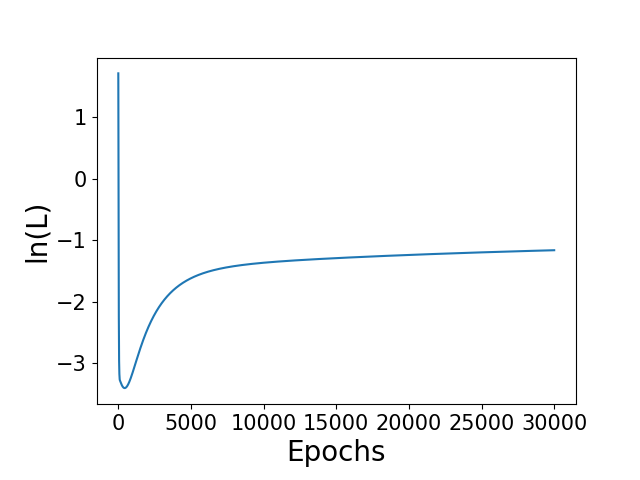
\includegraphics[width=\linewidth]{figures/loss_Sigmoid_30000.png}
                \caption{\emph{Plot of the natural log of the loss function against the number of epochs when using Sigmoid in the hidden layers of the neural network. This is the loss during the training phase as the neural network predicts the function sin(x) with a learning rate of 0.00002.}}
                \label{fig:9}
            \end{figure}

            Sigmoid performs considerably worse as an activation function than ReLU and tanh for the given hyperparameters. We analysed the mathematical properties of the Sigmoid function and its derivative to best understand the reason why Sigmoid performs poorly in this multi-layer neural network. It is instructive to compare it to tanh; as both functions exhibit similar properties. In fact, tanh can be expressed in terms of Sigmoid by scaling and translating the Sigmoid function as\cite{activation}
            \begin{equation}
                \tanh(x) = 2\sigma(2x) - 1.
            \end{equation}
            From this relationship, both functions are susceptible to having a vanishing gradient for large inputs ($\mid$$x$$\mid >> 1$). Often, non-zero centred activation functions can lead to undesirable results since the outputs are either all positive or all negative. From equation \ref{eq:dldw} therefore, the sign of the loss gradient with respect to the weight matrix is solely dependent on the sign of the loss gradient with respect to the output, since each component of the input is the same sign as a result of the non-zero centred activation function. The updates in the weights become imbalanced between positive and negative values, and this has the overall effect of slowing down learning. To counteract this, the weights were initially normalised between values -0.5 and 0.5. 

            Since the normalisation of the weights is zero-centred, it is now beneficial to compare the derivatives of Sigmoid and tanh in order to explain the difference in performance demonstrated by figures \ref{fig:9} and \ref{fig:7:b}. For values of $x$ that satisfy the inequality $\mid$$x$$\mid < 1.66$, the derivative of tanh is greater than the derivative of Sigmoid; and at $x = 0$ , it is exactly four times as large. Since it is sharply peaked about $x = 0$, input values close to zero result in a considerably larger value for equation \ref{eq:input_gradient_activation}. These larger gradient values ultimately lead to bigger updates in the weights and therefore explain why tanh learns far faster, and performs better than Sigmoid.

            To provide evidence for this explanation, we trained the neural network once again with Sigmoid as the activation function, but instead the learning rate was chosen to be 0.002. Increasing the learning rate should aid the the performance of the neural network by making stronger updates of the weights upon each step. 

            \begin{figure}
                \centering
                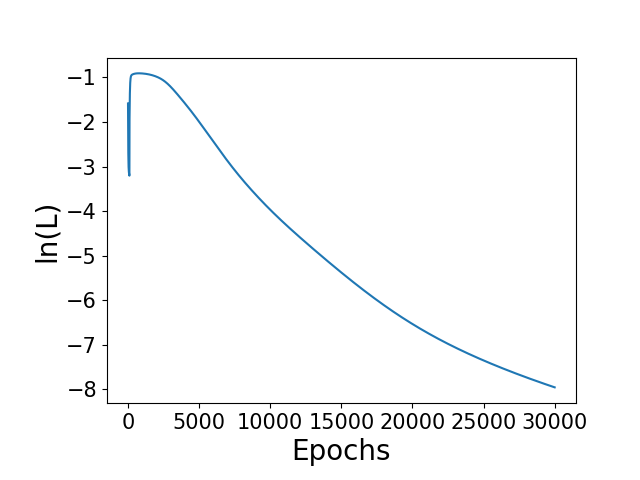
\includegraphics[width=\linewidth]{figures/loss_sigmoid_30000_0.02.png}
                \caption{\emph{Plot of the natural log of the loss function against the number of epochs when using Sigmoid in the hidden layers of the neural network. This is the loss during the training phase as the neural network predicts the function sin(x) with a learning rate of 0.002}}
                \label{fig:10}
            \end{figure}

            It is clear from figure \ref{fig:10} that the neural network using Sigmoid performs far better with the increased learning rate. This time, over $30,000$ epochs, the natural log of the loss function reaches its global minimum of $\ln(L) = -8$ once the training phase has concluded. Increasing the learning rate is not always beneficial for improving performance since if the learning rate is too high, the loss function can diverge or the neural network could over-fit to the training data; and fail to make accurate predictions on unseen test data. 

        \subsection{Book Genre Classification Results}

            In order to classify books genres, we implemented the use of a fully connected neural network (FCNN) which is ideal when dealing with vectorised data. We trained our machine learning algorithm on the data sourced from Open Library and used two separate embedding techniques as a way to compare the success of our results. The embedding techniques we used are Doc2Vec and sentence transformers (SBERT). As a way to depict our results, we recorded both accuracy and loss of both the training data and the validation data. The loss function used here is binary cross entropy (\ref{bce}) as it allows multiple genres to be predicted for each book.

            \begin{figure*}
                \centering
                \panel[0.48\textwidth]{bookacc:a}{figures/books_doc2vec_train_val_acc.png}\hfill
                \panel[0.48\textwidth]{bookacc:b}{figures/books_sbert_train_val_acc.png}
                \caption{\emph{Both training and validation accuracy were plotted over 10 epochs for the embedding methods Doc2Vec $(a)$ and SBERT $(b)$.}}
                \label{bookacc}
            \end{figure*}

            The graph depicted in figure \ref{bookacc:a} shows how the training accuracy using Doc2Vec approximately gets $95\%$ by the tenth epoch while the validation accuracy is approximately a constant $92\%$ but with more noticeable fluctuation in accuracy at earlier epochs. Alternatively, the graph in figure \ref{bookacc:b} shows how the training accuracy using the SBERT model is approximately $97\%$ by the tenth epoch and the validation accuracy for SBERT is roughly $94\%$ for its duration. The smaller gap between validation and training accuracies implies that SBERT has better generalisation for unseen data. Additionally, the steeper gradient in training accuracy suggests that the SBERT model also trains faster than the neural network using Doc2Vec.

            \begin{figure*}
                \centering
                \panel[0.48\textwidth]{bookloss:a}{figures/books_doc2vec_train_val_loss.png}\hfill
                \panel[0.48\textwidth]{bookloss:b}{figures/books_sbert_train_val_loss.png}
                \caption{\emph{The graphs here show the loss for training and validation for our Doc2Vec model (a) and our SBERT model (b).}}
                \label{bookloss}
            \end{figure*}

            The graph in figure \ref{bookloss:a} shows that over the first 2 epochs, training loss for the Doc2Vec model decreases rapidly only to slow its descent for the latter epochs, resulting in a value of $1.3$ after 10 epochs. Validation loss generally increases over the epochs and, after 10 epochs, gives a value of approximately $2.2$. Figure \ref{bookloss:b} shows a graph where the training loss for SBERT reaches approximately $0.85$ after 10 epochs, lower than that of the Doc2Vec model which implies that SBERT was more effective at fitting the data during the training phase. It also shows us that, after 10 epochs, the validation loss reaches a value of $1.5$ which is again lower than the same value for Doc2Vec, telling us that SBERT generalises better than its counterpart. Both models have decreasing loss in the training phase and,  while initially decreasing over the first two epochs, an increasing loss over time during the validation phase. After ten epochs, both graphs have a low training loss and a high validation loss, this implies that both models are over-fitting.

        \subsection{Handwriting Recognition Results}

            Alongside classifying book genres, the other work package we decided to undertake was to classify images using both a fully connected neural network (FCNN) and a convolutional neural network (CNN). To be more specific, we trained the neural networks using the MNIST dataset to classify letters and numbers; as well as training both neural networks to recognise a variety mathematical symbols. The two main metrics for measuring performance are accuracy and loss, and we have investigated how these metrics vary whilst the neural networks were being trained as well as during the validation process. We have also applied two different optimisation algorithms (Stochastic gradient descent and Adam) and compared how both accuracy and loss differs when using each one for the two neural networks. 

            \subsubsection{MNIST Dataset Results}

            \begin{figure*}
                \centering
                \panel[0.48\textwidth]{mnistacc:a}{figures/mnist_compare_acc.png}\hfill
                \panel[0.48\textwidth]{mnistacc:b}{figures/mnist_val_loss_compare.png}
                \caption{\emph{Figure displaying how the both accuracy $(a)$ and loss $(b)$ vary over 20 epochs during the validation process. Both FCNN and CNN have been trained on the MNIST dataset and a fraction of this dataset has been used as validation data. The two plots show the variation of accuracy and loss for the FCNN with optimisation algorithms stochastic gradient descent (blue curve) and Adam (orange curve), as well as for the CNN with Adam (green curve). The hyperparameters were initialised as $\alpha = 0.01$ (for Adam and SGD), $\beta_1 = 0.9$ and $\beta_2 = 0.99$. Softmax activation function has been used in the output layer and ReLU has been used as the activation function in all hidden layers for both neural networks.}}
                \label{mnistacc}
            \end{figure*}

            As indicated in figure \ref{mnistacc:a} the accuracy achieved by the FCNN with Adam on the validation dataset is the greatest with a value of 96\%. The FCNN with stochastic gradient descent and the CNN with Adam finalise on accuracies of 94\% and 82\% respectively. The plot depicting the loss (figure \ref{mnistacc:b}) provides further insight into how well the neural networks generalise to the unseen test data. Evidently, examining both the accuracy and the loss, the FCNN with stochastic gradient descent generalises the best to the unseen data. Both the accuracy and loss converge over the entirity of the validation process and this indicates that the neural network does not over-fit to the training data. Changing the optimiser to Adam for the FCNN ultimately achieved a greater accuracy than using SGD, and in fact the accuracy using Adam surpassed the final accuracy using SDG after the first epoch. However, the loss seems to diverge over the 20 epochs and this could be a sign of the neural network over-fitting to the training data. As a way to investigate this further, it is instructive to compare the loss during the training phase with the loss during the validation phase.

            \begin{figure*}
                \centering
                \panel[0.48\textwidth]{FCNNloss:a}{figures/mnist_fc_sgd_loss.png}\hfill
                \panel[0.48\textwidth]{FCNNloss:b}{figures/mnist_fc_adam_loss.png}
                \caption{\emph{Figure displaying how the loss varies with the number of epochs for the FCNN with stochastic gradient descent $(a)$ and Adam $(b)$ as optimisers. The loss during the validation phase is represented by the blue curve and the loss during the training phase is represented by the orange curve.}}
                \label{FCNNloss}
            \end{figure*}

            In figure \ref{FCNNloss:b}, the loss curve for the training phase appears to converge to value of 0.1 after 20 epochs, whereas the loss curve for the validation phase diverges as the number of epochs increases. When using SGD in figure \ref{FCNNloss:a}, the loss converges to approximately 0.2 after both the training and validation phases. Adam is an adaptive optimiser and shows much faster progress over the first few epochs when it comes to increasing accuracy and minimising loss. However, the validation accuracy plateaus and the validation loss diverges from the training loss and therefore this suggests that FCNN over-fits to the training data. Despite a slow convergence, the FCNN with stochastic gradient descent generalises well to the unseen validation data, and this is reflected in the increasing accuracy as well as the both the training and validation loss converging to approximately the same value.

            Figure \ref{mnistacc:a} and \ref{mnistacc:b} suggests that the CNN with the Adam optimiser has the poorest performance after the 20 epochs. After 6 epochs, the CNN performs well reaching an accuracy greater than 96\% but then fluctuates and declines for the reminder of the validation phase. To find an explanation for this drop in accuracy, it is instructive to compare the accuracy during the training phase with the accuracy during the validation phase.

            \begin{figure}
                \centering
                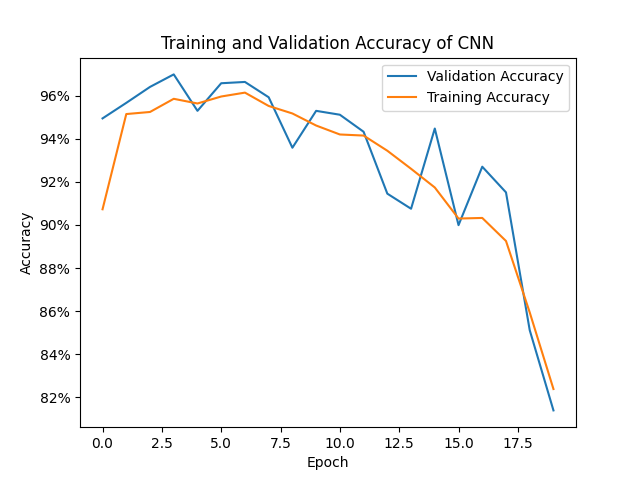
\includegraphics[width=\linewidth]{figures/mnist_cnn_acc.png}
                \caption{\emph{Plot displaying how the accuracy of the CNN using Adam varies with the number of epochs during the training (orange curve) and validation (blue curve) phases.}}
                \label{fig:14}
            \end{figure}

            The variation of accuracy with respect to the number of epochs for the validation phase exhibits the same decline as the accuracy for the training phase but with larger fluctuations. Typically, neural networks with convolution layers perform exceptionally well at image classification tasks; and this is the case for our CNN after the first 6 epochs. The decline in accuracy for both training and validation phases strongly suggests the neural network has been overtrained and has therefore passed the optimal number of training epochs for the selected hyperparameters. In order to achieve a more desirable performance using the validation data, we could run the CNN for only a few epochs (4-6), before the training accuracy decreases. The instability in the training and validation accuracies also suggest that initial hyperparameters such as learning rate is too high; and hence the drop in accuracy could be attributed to the CNN overfitting to certain parts of the data. Even though Adam uses an adaptive learning rate, it is still important that the initial values of the hyperparameters are tuned such that the CNN can achieve optimal performance.

            \subsubsection{Mathematical Symbol Classification Results}

            The performance of the neural networks can depend on the nature of the training and validation data as well optimisation algorithms, hyperpararmetrs and activation functions. We also tasked the same CNN and FCNN to perform image classification on a dataset of mathematical symbols. 

            \begin{figure}
                \centering
                \begin{center}
                    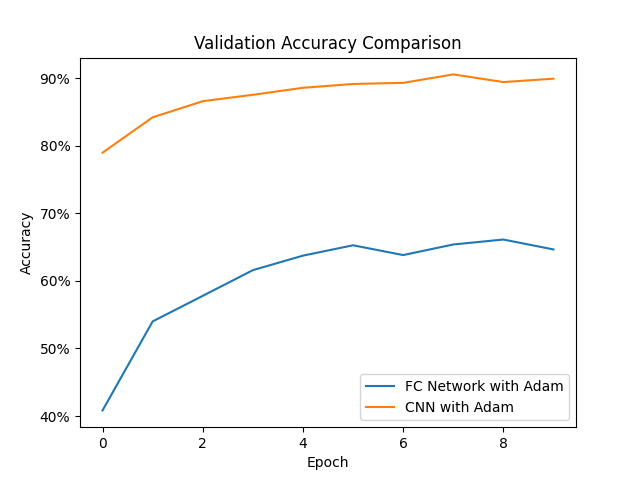
\includegraphics[width=\linewidth]{figures/math_acc_compare_500_10.png}
                    \caption{\emph{Plot displaying how the accuracy of the CNN (orange curve) and FCNN (blue curve) with the Adam optimiser varies over 10 epochs during the validation process.}}
                    \label{fig:15}
                \end{center}
            \end{figure}

            When comparing with the results from the MNIST dataset, the CNN greatly outperforms the the FCNN, and both neural networks appear to converge with final accuracies of 90\% and 65\% respectively. The validation accuracy is high after 1 epoch and gradually increases over the 10 epochs, stabilising at 90\%. The plateau in this case indicates that the CNN has learned the useful patterns in the data and has reached its performance limit. Figure \ref{fig:15} and the MNIST results both suggest that the CNN is far more efficient at spatial feature extraction as the validation accuracy reaches high values after over the first few epochs. The user-chosen parameters on the mathematical symbol data lead to a much more stable performance for the CNN over an extended number of epochs as the accuracy shows no sign of declining or fluctuation. The FCNN on the hand performs significantly worse on this dataset; showing a slower convergence and significantly lower final accuracy. Confirmation of both neural networks converging is evidenced by examining the variation of the loss over the training and validation phases.

            \begin{figure*}
                \centering
                \panel[0.48\textwidth]{Mathloss:a}{figures/math_loss_conv_500_10.png}\hfill
                \panel[0.48\textwidth]{Mathloss:b}{figures/math_loss_fc_500_10.png}
                \caption{\emph{Figure displaying how the loss varies with the number of epochs for the CNN (a) and FCNN (b) with Adam as the optimiser. The loss during the validation phase is represented by the blue curve and the loss during the training phase is represented by the orange curve.}}
            \end{figure*}

            For both neural networks, the loss for the validation and training phase both converge to a similar value. This ultimately demonstrates the neural network has trained successfully and there is no sign of over-fitting, thus the model generalises well to unseen data; achieving a similar accuracy on both training and validation data. The loss and accuracy are inversely related and hence the loss in figure \ref{Mathloss:b} converges to a value for greater than in figure \ref{Mathloss:a}.

            For both of the results obtained, the user-chosen parameters were initialised with the same values.  However, the loss function for the CNN and FCNN with Adam demonstrates convergence when making predictions on the maths symbols validation dataset, but appears to diverge when fed the MNIST validation data. Evidently, for the given hyperparameters, the specifics of the training and validation impact the performance of the neural network. The FCNN with stochastic gradient descent is a more simplistic model compared to the CNN, and achieves convergence after only 20 epochs on the MNIST data. This suggests that it is far easier for neural networks to learn on MNIST data than the the maths symbols data and it is likely that this is because the mathematical symbols are less distinctive. Therefore, the CNN with Adam is learning at such a high rate that it is over-fitting part of the training data and this could explain the large drop in accuracy for both the training and validation phases.

            

            \begin{figure*}
                \centering
                \panel[0.48\textwidth]{newloss:a}{figures/mnist_cnn_acc_lr005.png}\hfill
                \panel[0.48\textwidth]{newloss:b}{figures/mnist_cnn_loss_lr005.png}
                \caption{\emph{Plot displaying how the accuracy (a) and loss (b) of the CNN using Adam varies with the number of epochs during the training (orange curve) and validation (blue curve) phases. The initial learning rate for the Adam optimiser has been set to 0.005.}}
            \end{figure*}

            In order to prevent the CNN from over-fitting to part of the MNIST training data, we changed the initial learning rate for the Adam optimiser to 0.005, and left all other hyperparameters unaltered.
            Reducing the initial learning rate introduces more stability into the accuracy of the predictions made by the CNN. The training accuracy continues to increase over the 20 epochs and   reaches a final value of greater than 98\%.  Likewise, the validation accuracy shows a shallow increase over the 20 epochs but with slight fluctuations and achieves an accuracy of approximate 97.5\%. With the adjusted learning rate, the CNN displays successful performance and generalisation using MNIST, as indicated by the high, stable training and validation accuracies; as well as the loss showing no signs of divergence in figure \ref{newloss:b}.    

     \section{Ethical and Practical Considerations}

        When training machine learning algorithms, it is crucial to use as much data on a given topic as possible. The more data used to train the model, the higher the capacity the model has to achieve higher accuracies in its predictions when tested with unseen data. For shorter projects such as this one, it is not possible to collect primary data of sufficient size for this purpose. Hence, publicly available databases must be used. However, there are certain considerations that must be taken first, such as reading through the terms of use to ensure that using the database for machine learning training is consented to by the owners of the data, making sure that using their data is legally acceptable. It is not ethical to use someone else's work without their permission, or to use it for a purpose that was not consented to. In our case,  the databases we used (Open Library, MNIST, CROHME) were all cleared for use in our project by reading through the terms of service on their respective websites. 

        % Furthermore, we collected some of our own data using a survey, to supplement the data from the CROHME database of mathematical symbols. To ensure we met ethical guidelines for this,  we made sure that the data stored after people filled this survey out was completely anonymised. This is important as it meant that, once the survey was completed, we would be unable to tell who had submitted which data, protecting their privacy and their right to anonymity. 

    \section{Future Work}

        Due to time constraints and limited resources, we choose to focus our efforts on creating handwriting recognition models for pre-segmented symbols and book classification models using proprietary embedding techniques. However, given future opportunity, we would like to explore the possibility of creating a handwriting recognition model to identify unsegmented equations and documents.
        This could have useful application to students and academics in the STEM field such as automatic conversion of written notes to latex, and automatic write-ups of lectures given on white/chalk boards. This could be achieved by employing a non machine learning pre-processing algorithm to segment symbols and classifying each segmented symbol using our model. Another method could be to create a different model capable of classifying entire documents using more advanced neural network techniques such as a recurrent neural network.

        To extend our research into book classification and natural language processing,
        given future opportunity, we would like to explore the creation of our own embedding model. To do this, we would implement our own version of Doc2Vec.
        Another area we would like to pursue is generative AI. A possible idea we had was to generate titles for books based on the description. This could be achieved by using an llm like model.
    
    \section{Summary}

        The overall aim of this project was to develop neural networks to perform image classification tasks on handwritten characters and mathematical symbols, as well as using natural language processing in order to classify book genres based on their descriptions. We investigated how the performance of neural networks varied by recording metrics such as accuracy and loss during both training and validation processes; to gain an insight into the neural network's generalisation capabilities. In addition to this, we implemented two different optimisers (Adam and stochastic gradient descent), comparing their respective convergence rates and exposing the benefits of an adaptive learning rate. Altering activation functions within hidden layers and selecting different initial values for the hyperparameters proved that tuning the neural network was crucial in order to achieve optimal performance.

        Activation functions are used within hidden layers of neural networks to introduce non-linearity; allowing the neural network to represent complex patterns in the input data. We used a fully connected neural network with stochastic gradient descent optimiser to plot data points of the function $\sin(x)$ on the interval $(0,2\pi]$ and analysed how loss and plots varied over 30,000 epochs when implementing ReLU, tanh and Sigmoid activation functions. The natural log of loss function converged to -12.5 when using ReLU with a learning rat of 0.00002. For this learning rate, the minimisation of the loss function was most efficient using ReLU and least efficient using Sigmoid; where the loss function failed to converge to a global minimum. Analysing the differences between the mathematical properties of the activation functions influenced our decision to reduce the learning rate to 0.002 to improve the performance with Sigmoid. After doing this, we found that the loss showed signs of converge after 30,000 epochs and reached a global minimum of $\ln(L) = -8$.
        
        For the book genre classification, we discovered that using SBERT as the embedding technique resulted in a higher accuracy (94\%) on the validation data than using Doc2Vec (92\%) after running for 10 epochs. We obtained these results using the Adam optimiser with an initial learning rate of 0.01. Using both embedding techniques, we observed the validation loss diverged from training loss; suggesting that the models had over-fit to the training data. To counteract this, we could re-run the model with a reduced initial learning rate, such that we achieve an ideal fit to the training data; and the models demonstrate improved performance when tasked to take in unseen data.

        For image classification, we trained and validated both a convolution neural network as well as a fully connected neural network. When classifying handwritten characters from the MNIST dataset, we found that the CNN and FCNN with Adam (and an initial learning rate of 0.01) reached validation accuracies of 96\% after the first 5 epochs. The accuracy achieved by the CNN displayed large fluctuations and decreased to 82\% after the full 20 epochs. Whereas for these initial hyperparameters, the FCNN with SGD achieved a final validation accuracy of 94\% and the validation loss demonstrated steady convergence, reaching a minimum of under 0.2. Once again, reducing the initial learning rate to 0.005 proved to enhance the performance of the CNN. The final validation accuracy we achieved using the updated hyperparametres was 98\%. The CNN with Adam was the most successful at classifying the mathematical symbols. The CNN achieved a final accuracy of 90\% on the validation data which was far superior to the 65\% reached by the FCNN. 

        Possible limitations of the models lie with the training data for the books and mathematical symbols. Within the training data, there were fewer specific classes than others and therefore the models could learn patterns for some classes more effectively. This could have the ripple effect of limiting the validation accuracy as the neural network's have not been fed sufficient training data for those particular classes. By implementing a website survey to collect handwritten mathematical symbols, we could have obtained more of the under-represented symbols and used them to supplement the training data as well as the validation data. 

\pagebreak

\addcontentsline{toc}{section}{References}
\setlength{\parskip}{0pt}
\bibliographystyle{unsrt}
\bibliography{ref}

\end{document}
